\documentclass{article}
\usepackage[utf8]{inputenc}
\usepackage{graphicx}
\usepackage{fancyvrb}
\usepackage[T1]{fontenc}
\usepackage{lmodern}
\usepackage{hyperref}
\usepackage{xcolor}
\usepackage{verbatim}
\usepackage{amsthm}
\usepackage{amsmath}
\usepackage{caption}
\usepackage{textcomp}

\newcommand{\resource}[1]{(Local copy saved to \texttt{#1})}
\newcommand{\tttilde}[0]{\textasciitilde{}}
\newcommand{\todo}[1]{{\color{blue}{TODO: #1}}}

\theoremstyle{definition}
\newtheorem{program}{Program}
\newtheorem{exercise}{Exercise}

\begin{document}

\section{Background}
This document aims to give an introduction to CUDA C programming for students who are new to the language. Provided alongside these notes are fully documented example programs, as well as exercises that usually involve modifying these programs.

Section \ref{sec/setup} will describe how to access the CUDA environment that's available on the SECS servers. Section \ref{sec/model} will summarize a few key features of CUDA programming model. Section \ref{sec/optimization} will show off more advanced optimization techniques available to a CUDA programmer. Finally, Section \ref{sec/applications} will present applications of CUDA to several classes of problems that are well-suited for the GPU.

\section{Setting up a CUDA Environment}
\label{sec/setup}

This section will describe how to configure a development environment that's suitable for compiling and executing CUDA programs. By default, this assignment will assume the use of the SECS Linux server \texttt{yoko}, which is installed with a Tesla K20Xm graphics card. An additional subsection at the end will point to some resources on how to harness a CUDA-enabled GPU on a personal computer.

\subsection{Accessing the SECS servers}

\begin{itemize}
\item 
For the following steps, you will need an SECS account. If you don't already have one, an SECS account can be requested here:

\url{https://oakland.edu/secs/technology-office/}

\item 
The SECS servers can be accessed when off-campus with the use of a VPN. SECS provides VPN software that is compatible with Windows, MacOS, and Linux. The official SECS instructions on how to set up the VPN can be found here:
    
\url{http://www.secs.oakland.edu/docs/pdf/vpn.pdf}

\resource{resources/secs-vpn.pdf}
    
\item 
Once the VPN is installed, configured, and enabled, the SECS servers can be accessed via SSH from a terminal. Connect to the server \texttt{yoko.secs.oakland.edu} using your SECS username and password using the command: 
\begin{verbatim}ssh USERNAME@yoko.secs.oakland.edu\end{verbatim}
You will be prompted for your SECS password before the connection is accepted.

\item 
Further documentation on the SECS servers, including those which have CUDA-enabled GPUs, can be found here:

\url{https://www.secs.oakland.edu/docs/pdf/linuxServers.pdf}

\resource{resources/secs-linuxServers.pdf}

\item 
If you already had files saved on the SECS network, you can run the \texttt{ls} command to view them after connecting to the server. 
\end{itemize}

\subsection{The CUDA environment}

The primary tool when developing a CUDA program is the Nvidia CUDA compiler, \texttt{nvcc}. On the \texttt{yoko} server, \texttt{nvcc} should have already been made available by default, which you can verify by running \texttt{which nvcc}. If successful, this command will show the location of \texttt{nvcc} on the filesystem.

\texttt{nvcc} is a compiler for the language \emph{CUDA C/C++}, which is a \emph{superset} of both the standard C and C++ languages. That is, \texttt{nvcc} is still able to compile any C or C++ program that a normal compiler for those respective languages could. The remainder of this assignment will only use CUDA C.

\begin{itemize}
\item
As a first test of \texttt{nvcc}, run the command \texttt{nano hello-world.c} to open the terminal's text editor and enter the following simple C program:

\begin{verbatim}
#include <stdio.h>

void main() {
  printf("Hello world!\n");
}
\end{verbatim}

\item
Save and close the file. (Recall that in the \texttt{nano} text editor, Ctrl+X attempts to close the current file, after first prompting you to save the file if it has changed.)

\item
Compile the program with \texttt{nvcc hello-world.c -o hello-world}. The command-line argument "\texttt{-o hello-world}" tells the compiler to write the executable output to the file \texttt{hello-world}. If the \texttt{-o} flag isn't given, \texttt{nvcc} will write the executable to the file \texttt{a.out} by default.

\item
Run the executable with the command \texttt{./hello-world}. You should see the output \texttt{Hello world!}, just as you would with when using a normal C compiler.
\end{itemize}

\subsection{Installing CUDA locally}
If you have a relatively new Nvidia GPU installed in a personal computer, it's likely CUDA-enabled, meaning you would be able to follow these assignments without needing to use the remote SECS server. This will require substantially more configuration than is necessary on an SECS server, but may be worthwhile for an interested student who plans to use CUDA beyond the scope of this class.

In order to follow the remainder of the assignment on a local environment, you will need to install the CUDA Toolkit. Instructions are provided by Nvidia and will depend on your operating system.

\begin{itemize}
\item 
A list of CUDA-enabled GPUs is provided by Nvidia here:

\url{https://developer.nvidia.com/cuda-gpus}

\item 
CUDA installation instructions for Windows:

\url{https://docs.nvidia.com/cuda/cuda-installation-guide-microsoft-windows/index.html}

\item
CUDA installation instructions for Linux:

\url{https://docs.nvidia.com/cuda/cuda-installation-guide-linux/index.html}
\end{itemize} 

Once the CUDA Toolkit is installed, add the \texttt{bin} subdirectory from the installation directory to your PATH variable. This will make the newly installed CUDA executables available from the terminal. If this has been done successfully, the terminal command \texttt{which nvcc} should correctly display the location of the CUDA compiler.

\section{The CUDA Programming Model}
\label{sec/model}

The goal of the CUDA programming model is to provide a high-level interface to the highly parallelizable computational power of a GPU. This section will summarize the underlying structure of each CUDA program by example, as well as give a method of profiling CUDA programs that will be used to compare them to their serial counterparts.

\subsection{Thread hierarchy}
A function that is to be executed on the GPU is generally called a \emph{kernel}. When a CUDA program calls a kernel function, the program must also allocate that kernel a certain number of threads. Each thread will then execute its own copy of that function, either in parallel or in sequence, according to the kernel's definition.

The threads assigned to a kernel are divided into blocks, where each block has the same number of threads. Thus, each thread is associated to both a block index, as well as a thread index within that block. This data can be accessed by device code using the following CUDA-specific global variables:
\begin{itemize}
    \item \texttt{blockDim.x} contains the number of threads in each block.
    \item \texttt{blockIdx.x} contains the executing thread's block number.
    \item \texttt{threadIdx.x} contains the executing thread's index within its block.
\end{itemize}

If $N$ threads are allocated, then each thread can use the above three values to compute its own globally unique \emph{thread ID} (written \texttt{tid} in this assignment) between $0$ and $N - 1$. This pattern is used frequently in CUDA programs: \begin{verbatim}int tid = blockDim.x * blockIdx.x + threadIdx.x;\end{verbatim} 

\begin{program}
Compile and execute \texttt{print-tid.cu} in your CUDA environment. You should get output similar to the following:
\\~\\
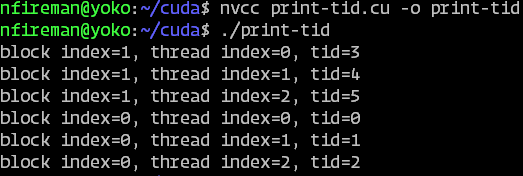
\includegraphics[width=\textwidth]{images/print-tid-output.png}

There are several language features of CUDA C to note about this program:
\begin{itemize}
\item 
    The \texttt{\_\_global\_\_} keyword indicates that the marked function executes on the device but is called from the host (in other words, the marked function is a kernel function). A similar keyword, \texttt{\_\_device\_\_}, means the marked function both executes on and must be called by the device.
    
\item 
    The triple angle bracket notation seen in \texttt{print\_tid<<<2,3>>>()} is known as a \emph{kernel launch}. Calling a kernel function in this way from the host means that 2 thread blocks that contain 3 threads will each call that kernel function (allocating 6  threads altogether).
    
\item 
    The \texttt{cudaDeviceSynchronize()} function blocks the program's process until each device thread has finished executing. Without this synchronization call, the host process may terminate before one or more threads has a chance to print its statement to the console.
    
\item
    Finally, note that each \texttt{tid} value printed to the console is unique and between 0 and 5, as expected. 
\end{itemize}
\end{program}

\begin{exercise}
Change the \texttt{print\_tid} kernel launch to use 4 blocks of 3 threads each, recompile and execute the program, and verify that the thread ID values are again unique from 0 to 11.
\end{exercise}

\subsection{Memory model}

In the context of a CUDA program, the CPU is known as the \emph{host} and the CUDA-enabled GPU is known as the \emph{device}. The host cannot directly access the device's memory (and vice versa); the memory of one must be copied to the memory of the other by calling a CUDA library function. Therefore, a CUDA program will often broadly consist of the following steps:
\begin{enumerate}
    \item Allocate sufficient memory on the device to store data needed for a computation.
    \item Copy the data from host memory to device memory.
    \item Perform a computation on the device using the data in device memory.
    \item Copy the results back from device memory to host memory.
\end{enumerate}

\begin{program}
The program \texttt{parallel-add.cu} illustrates these steps in a minimal CUDA program. Run and compile the \texttt{parallel-add.cu} program and compare your observed output to the following:

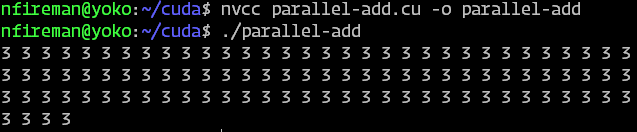
\includegraphics[width=\textwidth]{images/parallel-add-output.png}

The program allocates \texttt{N} threads on a single block, and performs one addition per thread in the kernel function \texttt{kernel\_add}. To verify that the program is working correctly, it prints the resulting sums after copying them from the device back to the host.

This program introduces the following features of CUDA C:
\begin{itemize}
\item 
The function \texttt{cudaMalloc} is the standard way to allocate device memory. Consider the call:
\begin{verbatim}int *dev_a;
cudaMalloc((void**)&dev_a, N * sizeof(int));\end{verbatim}
    
    \begin{itemize}
    
    \item 
    The second argument \texttt{N * sizeof(int)} denotes the number of bytes of device memory to allocate.
    
    \item 
    The value \texttt{\&dev\_a} is the address of the pointer \texttt{dev\_a}. Its address is passed instead of the value itself since \texttt{cudaMalloc} will write the pointer to allocated device memory into the address of \texttt{dev\_a}, changing its value. This is known as a \emph{pass by reference}.
    
    \item 
    Since \texttt{dev\_a} is of type \texttt{int*}, \texttt{\&dev\_a} will be of type \texttt{int**}, as \texttt{\&dev\_a} is a pointer to \texttt{dev\_a}. However, since \texttt{cudaMalloc} is written to allocate any amount (that is, any type) of memory, it expects its pointer argument to be of type \texttt{void**}, which signifies a pointer to \emph{typeless} memory. To accommodate this, \texttt{\&dev\_a} must be cast to \texttt{void**}.
    
    \item 
    Once \texttt{dev\_a} has been set to a device memory pointer by \texttt{cudaMalloc}, it is an error to attempt to read its value on the host. In order to read device memory from the host, a suitable function from the CUDA API must be used. 
    \end{itemize}
    
\item 
The function \texttt{cudaMemcpy} is used both to copy memory from device to host and vice versa. Consider the two calls:
\begin{verbatim}cudaMemcpy(dev_a, a, N * sizeof(int), cudaMemcpyHostToDevice);
cudaMemcpy(c, dev_c, N * sizeof(int), cudaMemcpyDeviceToHost);
\end{verbatim}
    \begin{itemize}
        \item 
        \texttt{cudaMemcpy} always copies from its second argument into its first argument.
        
        \item
        The third argument \texttt{N * sizeof(int)} states the number of bytes of memory to copy. 
        
        \item 
        The fourth argument describes whether the source and destination memory are on the device or host using a value from the enum \texttt{cudaMemcpyKind}. In particular, note that \texttt{cudaMemcpyHostToHost} and \texttt{cudaMemcpyDeviceToDevice} also exist, though their use is less common.
        
        \item
        Thus, the first call above copies \texttt{N int} values from \texttt{a} on the host to \texttt{dev\_a} on the device. Likewise, the second call copies \texttt{N int} values from \texttt{dev\_c} on the device to \texttt{c} on the host.
    \end{itemize}
    
\item
Finally, note the usage of the thread ID (\texttt{tid}) in the kernel function to assign each thread a unique piece of the overall program's computation.
\end{itemize}

\end{program}

\begin{exercise}
Modify \texttt{parallel-add.cu} so that the size of the arrays \texttt{a}, \texttt{b}, and \texttt{c} is twice the number of threads. Then, modify the kernel function so that each thread performs two additions on its input arrays instead of just one. Make sure that no two threads perform an addition on the same array index.
\end{exercise}

\subsection{Events and timing}

A common theme in this assignment will be to compare the performance of a regular C program with a parallelized CUDA program that performs the same task. This will be accomplished by comparing the runtimes of the C program to that of the equivalent CUDA program. 

Timing CUDA program execution is best done using a language feature known as \emph{CUDA events}. For our purposes, a CUDA event is a timestamp at a certain point in the device's execution. 

\begin{program}
The program \texttt{parallel-add-timed.cu} builds on the previous \texttt{parallel-add.cu} program by using CUDA events to time the execution of the \texttt{kernel\_add} kernel. In addition to the output of the original \texttt{parallel-add} program, this program also prints the duration of the kernel execution.

Run and compile the \texttt{parallel-add-timed.cu} program and compare your observed output to the following:

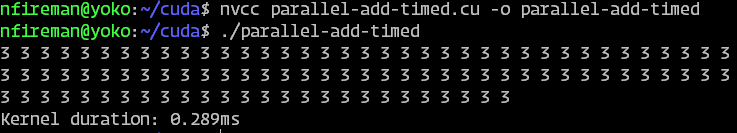
\includegraphics[width=\textwidth]{images/parallel-add-timed-output.png}

The following features of CUDA events are introduced by this program:

\begin{itemize}
    \item 
    The type of a CUDA event is \texttt{cudaEvent\_t}.
    
    \item
    Each CUDA event must be \emph{created} by passing it to \texttt{cudaEventCreate} before it can be used.
    
    \item 
    Passing an event to the function \texttt{cudaEventRecord} saves a timestamp in that event. This is used both before and after the kernel is executed to save timestamps in the events \texttt{start} and \texttt{stop}, respectively.
    
    \item
    The call \texttt{cudaEventSynchronize(stop)} blocks the host until the \texttt{stop} event has been recorded (that is, passed to \texttt{cudaEventRecord}). This serves the same purpose as \texttt{cudaDeviceSynchronize()}, which was used previously.
    
    \item
    The duration between the two recorded events is computed with the call \texttt{cudaEventElapsedTime(\&milliseconds, start, stop)}. Note that the computed duration is returned by reference using the first \texttt{float} argument, rather than as the return value of the function call itself.
    
    \item
    The function \texttt{cudaEventDestroy} is used to free an event's memory after the event isn't needed anymore. While this is an important step in large, real-world programs to avoid memory leaks, in simple example programs like this one it's ultimately unnecessary.
\end{itemize}
\end{program}

\begin{exercise}
\label{ex-timed-1}
Note that the addition in the kernel function of \texttt{parallel-add-timed} is nested in a for loop, where the number of loop iterations is equal to \texttt{TRIALS}. By default, \texttt{TRIALS} is set to 1. Recompile and execute the program again where \texttt{TRIALS} is set to 10, 1,000, and 100,000, and record the resulting duration in each case. Does the duration increase at the same rate as the number of trials?
\end{exercise}

\begin{exercise}
The program \texttt{serial-add-timed.c} has been provided to perform a comparable task as \texttt{parallel-add-timed.cu}, except without the use of CUDA. Use the command
\begin{verbatim}gcc serial-add-timed.c -o serial-add-timed\end{verbatim} 
to compiler this program with the \texttt{gcc} C compiler. Compare its execution time to that of \texttt{parallel-add-timed.cu} where \texttt{TRIALS} is set to 10, 1,000, and 100,000.
\end{exercise}

\begin{exercise}
The constant \texttt{N} in both \texttt{parallel-add-timed.cu} and \\
\texttt{serial-add-timed.c} determines the length of the arrays being added. Compare the execution times after changing the value of \texttt{N} in both programs to 10,000, 100,000, and 1,000,000 (while \texttt{TRIALS} is still set to 1, as in the original programs).

\textbf{Note:} you should also remove the \texttt{for} loop at the end of the \texttt{main} function that prints every element of the result array for large values of \texttt{N}.
\end{exercise}

\section{Optimization techniques}
\label{sec/optimization}
\subsection{Shared block memory}
\label{subsec/shared-block-memory}
As you may know, modern CPU memory is organized in a \emph{memory hierarchy}, which ranks a system's memory by its access speed. Processors can take advantage of even a small amount of fast memory by copying data to it, manipulating the faster memory, then copying results back to the slower, larger memory. 

The CUDA platform also adheres to this principle by way of \emph{shared memory}, which is a small amount of fast memory that is shared by the threads in a thread block. At a high level, a thread block's shared memory is located on the same chip as the GPU cores acting as the threads in that block; this is known as \emph{on-chip memory}. For this reason, the shared memory has higher \emph{bandwidth} (rate of transfer) and lower \emph{latency} (time for a transfer to complete) than the \emph{global memory} that we have used until now. In particular, when \texttt{cudaMemcpy} is used in the \texttt{cudaMemcpyHostToDevice} mode, the host memory is being copied into the device's global memory.

To demonstrate the effectiveness of shared memory, we will compare the execution times of two programs that complete the same task, where one program's kernel uses shared memory and the other uses only global memory. Both programs compute the \emph{dot product} of two arrays \texttt{a} and \texttt{b} of length \texttt{N}, which is defined as:
\begin{verbatim}
dot_prod = (a[0] * b[0]) + (a[1] * b[1]) + ... + (a[N-1] * b[N-1])
\end{verbatim}

Since each of the \texttt{N} terms of this sum can be computed independently of each other, this computation can be parallelized in a straightforward yet highly effective way, as follows. Each allocated thread will be assigned certain indices between \texttt{0} and \texttt{N}. For each such index \texttt{i} assigned to it, that thread will compute \texttt{a[i] * b[i]}, writing the result to another array at \texttt{c[i]}. Once all products have been computed, the elements of the array \texttt{c} can be summed by the host to arrive at the desired dot product. This will be the approach used by the kernel that only uses global memory.

To take advantage of shared memory in a second approach, each thread will maintain its own \emph{partial sum} equal to the sum of the \texttt{a[i] * b[i]} terms that thread was assigned to compute. Each thread will then write its partial sum into shared memory, and one thread in each block will be assigned the additional task of summing these per-thread partial sums to compute a per-block partial sum, which can finally be written to global memory. The host will sum the block-wide partial sums to arrive at the desired dot product as before. 

Note that the main improvement in the latter shared memory approach comes from decreasing the number of writes made to global memory. The first approach needs to write once to global memory for each index of the input arrays, while the second approach only needs to write to global memory once per thread block.

\begin{program}
The above dot product algorithms are implemented in\\ \texttt{dot-product-globalmem.cu} and \texttt{dot-product-sharedmem.cu}. The latter program uses shared memory, introducing the following new features of CUDA C:

\begin{itemize}
    \item The \texttt{\_\_shared\_\_} keyword is used in a variable declaration to denote its allocation in shared memory. Thus, the net effect of the statement
    \begin{verbatim}__shared__ float threadPartials[THREADS_PER_BLOCK];\end{verbatim}
    is to allocate one such array for each thread block associated to the kernel launch.
    
    \item Since shared memory is shared by \emph{every thread in a thread block}, and is therefore vulnerable to race conditions, should one thread write to a location in shared memory that another thread can possibly read or write from in a nondeterministic order.
    
    \item The \texttt{\_\_syncthreads()} function is another example of a synchronization barrier, as we have seen previously with \texttt{cudaEventSynchronize} and \\ \texttt{cudaDeviceSynchronize}. Calling \texttt{\_\_syncthreads()} from the device will force the caller's thread to wait until every other thread in its block has also called \texttt{\_\_syncthreads()}. Thus, \texttt{\_\_syncthreads} is an essential tool when using shared memory to avoid race conditions as described above.
    
    In \texttt{dot-product-sharedmem.cu}, the call to \texttt{\_\_syncthreads()} is used to wait until the shared memory array \texttt{threadPartials} has received every thread's partial sum, at which point it is safe to compute the per-block partial sum.
\end{itemize}
\end{program}

\begin{exercise}
Currently, \texttt{dot-product-sharedmem.cu} computes the dot product of two \texttt{float} arrays. Modify the program so that it computes the dot product of two \texttt{int} arrays. In the modified program, the kernel function should have the signature:
\begin{verbatim}
__global__ void kernel_dot(int* a, int* b, int* blockPartials)
\end{verbatim}
After modifying the program and confirming that it still correctly computes the dot product, compare its execution time to the original program that used \texttt{float} arrays.
\end{exercise}

\subsubsection*{Additional resources}
\begin{itemize}
    \item Section 3.2.4 (Shared Memory) of the CUDA C Programming Guide:
    
    \url{https://docs.nvidia.com/cuda/cuda-c-programming-guide/index.html#shared-memory}
    
    \resource{resources/CUDA\_C\_Programming\_Guide.pdf}
    
    \item A brief NVIDIA blog post introducing the performance benefits of CUDA shared memory:
    
    \url{https://developer.nvidia.com/blog/using-shared-memory-cuda-cc}
    
    \resource{resources/Using\_Shared\_Memory.pdf}
    
    \item Section 5.3 of "CUDA by Example: An Introduction to General-Purpose GPU Programming" by Jason Sanders Edward Kandrot

\end{itemize}

\subsection{Atomic operations}

In a multithreaded program, an operation on a value is \emph{atomic} if only one thread is allowed access to that value while the atomic operation is in progress. Atomic operations are necessary when many concurrent threads are trying to read or write to the same value. The CUDA environment provides atomic versions of several arithmetic operations that can be used to perform atomic operations in a CUDA program.

To demonstrate the use of atomic operations in CUDA, two programs are provided whose kernel functions compute a \emph{histogram} representing random numerical data. That is, given the input array of integers \texttt{values}, both kernels compute a histogram array \texttt{histo}, where at the end of the kernel execution, \texttt{histo[i]} is equal to the number of times the integer \texttt{i} appears in \texttt{values}. Histograms are best known as a tool to summarize data in a human-readable way, but they also have algorithmic applications in image processing and computer vision.

To compute the histogram of the input array, each thread iterates over its own share of input values read from \texttt{values}. For each input value, the thread must record its presence in the histogram \texttt{histo} by performing the following steps:
\begin{enumerate}
    \item Read the current value of \texttt{histo[i]}.
    \item Compute the value \texttt{histo[i] + 1}.
    \item Overwrite \texttt{histo[i]} with the value \texttt{histo[i] + 1}.
\end{enumerate}
If these steps aren't guaranteed to be atomic, then two  threads may read \texttt{histo[i]} before the other can write the incremented value. This results in both threads setting the value to \texttt{histo[i] + 1}, even though two increments should have taken place. Thus, the histogram kernel needs to be able to perform atomic additions to the integer values currently stored in \texttt{histo}.

Atomic addition in CUDA is performed with the call: \begin{verbatim}atomicAdd(int* address, int value)\end{verbatim}
which atomically adds \texttt{value} to the integer located at the address \texttt{address}. Note that differently-typed versions of \texttt{atomicAdd} exist for \texttt{float}, \texttt{double}, and so on, but they are all named \texttt{atomicAdd}.

\begin{program}
The programs \texttt{histogram-globalmem.cu} and \\ \texttt{histogram-sharedmem.cu} are provided to demonstrate the use of atomic operations in CUDA.

In \texttt{histogram-globalmem.cu}, each thread performs an \texttt{atomicAdd} operation on an element of the histogram \texttt{histo} for each input value that thread processes. Thus, the number of concurrent \texttt{atomicAdd} operations at any one time is limited to the number of entries in \texttt{histo}, since each entry supports at most one atomic addition at a time.

The program \texttt{histogram-sharedmem.cu} resolves this issue with the aid of shared memory. Each block of threads computes its own per-block histogram \texttt{histo\_block}, summarizing the values processed by the threads in that block. Each \texttt{histo\_block} array supports as many concurrent atomic additions as it has entries as before, and there are as many such arrays as there are allocated thread blocks. Thus, the maximum possible concurrency is increased by a factor of the number of allocated blocks when compared to \texttt{histogram-globalmem.cu}.

Of course, once a thread block finishes computing its own \texttt{histo\_block}, it must atomically add those values to the output histogram \texttt{histo} in global memory. 
\end{program}

\begin{exercise}
Compile and execute \texttt{histogram-globalmem.cu} and\\
\texttt{histogram-sharedmem.cu} and compare their execution times. 
\end{exercise}

\begin{exercise}
Modify both \texttt{histogram-globalmem.cu} and\\
\texttt{histogram-sharedmem.cu} to use an input array of size 10,000 by changing the value of \texttt{N} in both programs. Compare the resulting execution times of both programs. Next, repeat the same process using the value 1,000,000 for \texttt{N}.
\end{exercise}

\begin{exercise}
In the kernel function of \texttt{histogram-sharedmem.cu},  several steps are currently performed by the one thread in each block with \texttt{threadIdx.x == 0} (namely, the first step that initializes \texttt{histo\_block} and the last step that adds \texttt{histo\_block} values to the output \texttt{histo} array in global memory). 

Modify the program so that the work done in those steps is evenly divided between the threads in each block, in the same way that the computation of the histogram itself is divided evenly between all threads in each block. Compare the execution time of your modified program to the original version of \texttt{histogram-sharedmem.cu}.
\end{exercise}

\subsubsection*{Additional resources}
\begin{itemize}
    \item Section B.14 (Atomic Operations) of the CUDA C Programming Guide:
    
    \url{https://docs.nvidia.com/cuda/cuda-c-programming-guide/index.html#atomic-functions}
    
    \resource{resources/CUDA\_C\_Programming\_Guide.pdf}
    
    \item Chapter 9 of "CUDA by Example: An Introduction to General-Purpose GPU Programming" by Jason Sanders, Edward Kandrot.
    
    \item Chapter 9 of "Programming Massively Parallel Processors: A Hands-on Approach", 3rd Edition by David B. Kirk, Wen-mei W. Hwu.
\end{itemize}

\subsection{Pinned host memory}

So far, we have allocated host memory using the standard \texttt{malloc} function in the C standard library. As a reminder, this memory has been allocated and copied to the device as follows:
\begin{verbatim}
int *a, *dev_a;
a = (int*)malloc(N * sizeof(int));
cudaMalloc((void**)&dev_a, N * sizeof(int));
cudaMemcpy(dev_a, a, N * sizeof(int), cudaMemcpyHostToDevice);
\end{verbatim}

The memory allocated by \texttt{malloc} is known as \emph{pageable memory}. This refers to the operating system's ability to \emph{page out} this data from RAM to the disk when it hasn't been recently used, which is done automatically by every modern operating system for performance reasons. One consequence of this is that the location of pageable memory in physical RAM may change, meaning it does not have a fixed address that can be referenced by other programs (such as a device kernel). 

As a result of this, the above code snippet will not cause the data on the host in the array \texttt{a} to be directly copied to the device. Instead, CUDA will first allocate temporary \emph{pinned memory} (also known as \emph{page-locked memory}), which cannot be paged out by the operating system to the disk and thus has a consistent address. CUDA will then copy the array \texttt{a} twice: first from its original location allocated by \texttt{malloc} to the temporary pinned memory, and second from the pinned memory to the device.

In order to avoid data being copied from pageable memory to pinned memory as described above, one can manually allocate pinned memory using the CUDA function \texttt{cudaMallocHost} instead of \texttt{malloc}:
\begin{verbatim}
int *a_pinned, *dev_a;
cudaMallocHost((void**)&a_pinned, N * sizeof(int));
cudaMalloc((void**)&dev_a, N * sizeof(int));
cudaMemcpy(dev_a, a_pinned, N * sizeof(int), cudaMemcpyHostToDevice);
\end{verbatim}

This will result in the array \texttt{a\_pinned} being copied only once: from its original allocation site on the host to the device. Note, however, that pinned memory that is manually allocated in this way must also be manually freed using the function \texttt{cudaFreeHost}. Since pinned memory will (by definition) remain in RAM until it is freed, pinned memory leaks can be very costly.

\begin{program}
The program \texttt{host-memory-comparison.cu} is provided to demonstrate the runtimes when using \texttt{cudaMemcpy} to copy data from both unpinned host memory and pinned host memory. Compile and execute the program. Compare your results to the following screenshot:

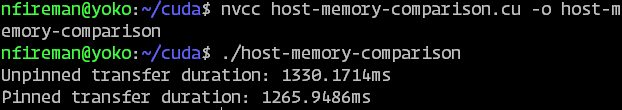
\includegraphics[width=0.9\textwidth]{images/host-memory-comparison-output.png}
\end{program}

\begin{exercise}
Modify \texttt{host-memory-comparison.cu} so that both arrays stored in unpinned and pinned host memory are initialized with random integers before they're copied to the device (for an example of how to generate random integers, refer to the histogram programs from an earlier section). Record the resulting runtimes. Are they noticeably different than the original program?
\end{exercise}

\begin{exercise}
Currently, the two tests in \texttt{host-memory-comparison.cu} only measure the time it takes for memory to copied from the host to the device. Modify the program so that both tests measure the time it takes to copy the memory from host to device, then copy the same memory back from the device to the host. Record the resulting runtimes.
\end{exercise}

\begin{exercise}
The NVIDIA blog post referenced in the resources at the end of this section provides its own program that is similar to \texttt{host-memory-comparison.cu}. Their program also compares the transfer times of pinned and unpinned host memory, but goes one step further by also computing the bandwidth of a large memory transfer from each type of host memory to the device.

Their program is provided as \texttt{nvidia-bandwidthtest.cu}. Compile and execute this program. Compare your observed output to the following screenshot:

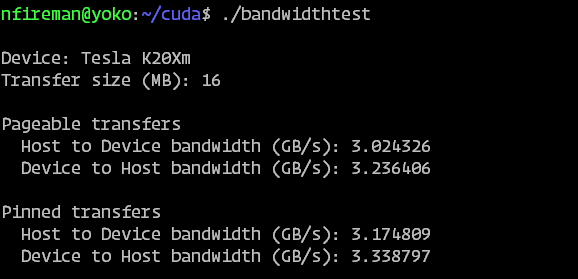
\includegraphics[width=\textwidth]{images/bandwidth-test-output.png}
\end{exercise}

\subsubsection*{Additional resources}
\begin{itemize}
    \item A brief NVIDIA blog post summarizing pinned host memory:
    
    \url{https://developer.nvidia.com/blog/how-optimize-data-transfers-cuda-cc/}
    
    \resource{resources/Optimize\_Data\_Transfers.pdf}
    
    \item Section 10.2 of "CUDA by Example: An Introduction to General-Purpose GPU Programming" by Jason Sanders, Edward Kandrot.
\end{itemize}

\section{Applications}
\label{sec/applications}
\subsection{Convolution filters}

A \emph{convolution} is a general mathematical operation that "blends" two functions together in some way to produce a third function. Convolutions have seen wide application in many fields, including image processing, where applying a  \emph{convolution filter} means transforming each pixel of an image based on what the image looks like near that pixel. For simplicity, we will be applying a convolution filter to a 1D array of pixel values, rather than the usual 2D array of pixels that comprises an image.

A convolution filter is characterized by its \emph{mask}, which is an array of values that define how much influence nearby pixels should have when applying the filter. As an example, suppose we have the following input array and mask:

\begin{verbatim}
int input_array[8] = {3, 1, 0, 2, 6, 3, 4, 1};
int mask[5] = {1, 2, 3, 2, 1};

// will hold the result from applying `mask` to `input_array`.
int output_array[8]; 
\end{verbatim}

Note that \texttt{output\_array} will always have the same size as \texttt{input\_array}. The \texttt{i}-th value of the output array \texttt{output\_array[i]} is computed as the dot product (defined in Section \ref{subsec/shared-block-memory}) of \texttt{mask} and a \texttt{mask}-sized subarray of \texttt{input\_array} that is \emph{centered} at index \texttt{i}. For example, the following line computes \texttt{output\_array[4]}:

\begin{verbatim}
output_array[4] = 1*0 + 2*2 + 3*6 + 2*3 + 1*4;
\end{verbatim}

In this example, we have computed the dot product of \texttt{mask} with \texttt{\{0,2,6,3,4\}}, which is the \texttt{mask}-sized subarray of \texttt{input\_array} centered at index 4.

One complication with this definition is when computing a value  like \texttt{output\_array[0]}, which is too close to the array boundary to fit a full \texttt{mask}-sized subarray centered there. In cases like these, we simply ignore the extra values of \texttt{mask} and \texttt{input\_array} that don't fit:

\begin{verbatim}
output_array[0] = 3*3 + 1*2 + 0*1;
output_array[1] = 3*2 + 1*3 + 0*2 + 2*1;
output_array[6] = 6*1 + 3*2 + 4*3 + 1*2;
output_array[7] = 3*1 + 4*2 + 1*3;
\end{verbatim}

\begin{program}
The program \texttt{convolution1.cu} implements the convolution filter algorithm described above. It uses a new feature of CUDA C, \emph{constant memory}, indicated by the \texttt{\_\_constant\_\_} modifier on the declaration of \texttt{dev\_mask}:

\begin{verbatim}
__constant__ int dev_mask[MASK_SIZE];
\end{verbatim}

This memory is "constant" in the sense that it cannot be modified from the device. Constant memory is initialized using \texttt{cudaMemcpyToSymbol}, which has an identical signature to \texttt{cudaMemcpy} that we have already used. The following line of code initializes the constant memory \texttt{dev\_mask} by copying the contents of \texttt{mask} into it:

\begin{verbatim}
cudaMemcpyToSymbol(dev_mask, mask, MASK_SIZE * sizeof(int));
\end{verbatim}

Note that there isn't an equivalent of \texttt{cudaMalloc} that allocates constant memory. The above variable declaration of \texttt{dev\_mask} performs this role. 

Compile and execute \texttt{convolution1.cu}. Compare your observed output to the following screenshot:

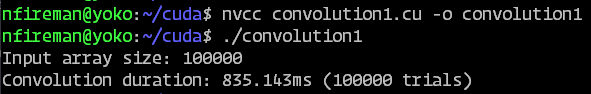
\includegraphics[width=\textwidth]{images/convolution1-output.png}

\end{program}

\begin{exercise}
Modify \texttt{convolution1.cu} so that the \texttt{mask} array is copied to global device memory and passed as an argument to \texttt{convolution\_kernel}, instead of using constant memory. Compare the performance of the modified program to the original.
\end{exercise}

\begin{program}
As shown in Section \ref{subsec/shared-block-memory}, shared memory can greatly improve the performance of a CUDA application when multiple threads in a block need to access the same data. The provided program \texttt{convolution2.cu} gives a second implementation of a convolution filter using shared memory. 

To take advantage of shared memory, one thread in each thread block is assigned to copy a so-called \emph{tile} of the input array into shared memory. The tile will contain all values in the input array that each thread in the thread block will need to compute its own output value. Because of how convolution filters are defined, two adjacent threads will access many of the same input values, and so almost all of the input values copied to shared memory will be accessed multiple times. By copying these values to shared memory \emph{once} before the convolution takes place, this program gains the benefit of shared memory \emph{multiple times}; once for each additional time the value is read.

You should find that the shared memory version applies convolution filters of the same size noticeably faster compared to the previous implementation:

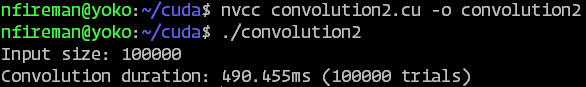
\includegraphics[width=\textwidth]{images/convolution2-output.png}
\end{program}

\begin{exercise}
The size of the mask in both convolution programs is defined by \texttt{MASK\_SIZE}. Record the runtimes when this value is modified to 11, 15, and 21 in both programs. Which runtime increases faster? Try to explain your findings.
\end{exercise}

\begin{exercise}
Currently, the shared memory array \texttt{tile} is initialized solely by the thread in each block where \texttt{threadIdx.x} is 0. Modify \texttt{convolution2.cu} so that the shared memory is initialized concurrently by all threads in each block.
\end{exercise}

\begin{exercise}
Currently in \texttt{convolution2.cu}, every input array value needed by a thread block is copied to the shared memory array \texttt{tile}. However, the values on the boundary of the tile won't be used as often as those not on the boundary. In fact, the first and last elements of \texttt{tile} will only be used by one thread in the block each (the first and last threads, respectively), so it's a net performance loss to copy these elements into shared memory.

Modify \texttt{convolution2.cu} so that \texttt{tile} has width equal to \texttt{THREADS\_PER\_BLOCK}, the number of threads in each thread block. In doing so, you should aim to maximize performance by reading input array values from global memory when they won't be needed by the maximum number of threads.
\end{exercise}

\subsubsection*{Kernel profiling with \texttt{nvprof}}

We have seen in several example programs how to use CUDA events to measure the execution durations of kernels. This section will briefly show how the profiling tool \texttt{nvprof}, provided as part of the CUDA environment, can be used to measure a kernel's execution duration automatically. By passing a compiled program to \texttt{nvprof}, the profiler will run the program and monitor its execution, producing a report that lists the share of execution time spent on each GPU activity and CUDA API call.

The following screenshot demonstrates the usage of \texttt{nvprof} to profile \texttt{convolution1.cu} (omitting the profiler's report for brevity). Note that the original program's output is printed, since \texttt{nvprof} executes the program to obtain its measurements.

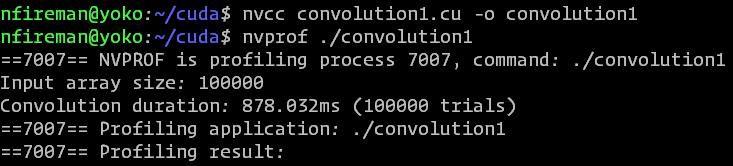
\includegraphics[width=\textwidth]{images/nvprof-output.png}

The report should list three rows with the type \texttt{GPU Activities}. One is named \texttt{convolution\_kernel(int*, int*, int, int)}, corresponding to the kernel function that applies the convolution filter. The other two rows are named \texttt{[CUDA memcpy HtoD]} and \texttt{[CUDA memcpy DtoH]}, which refer to host-to-device and device-to-host memory transfers, respectively.

\begin{exercise}
Use \texttt{nvprof} to measure the execution time of the kernels in \texttt{convolution1.cu} and \texttt{convolution2.cu}. Compare the results to the execution times printed by the programs themselves that were computed using CUDA events.
\end{exercise}

\subsubsection*{Additional resources}
\begin{itemize}
    \item Chapter 7 of "Programming Massively Parallel Processors: A Hands-on Approach", 3rd Edition by David B. Kirk, Wen-mei W. Hwu.
    
    \item "Image Convolution with CUDA" by Victor Podlozhnyuk.
    
    \url{http://developer.download.nvidia.com/compute/cuda/1.1-Beta/x86_64_website/projects/convolutionSeparable/doc/convolutionSeparable.pdf}
    
    \resource{resources/convolutionSeparable.pdf}
    
    \item NVIDIA documentation for \texttt{nvprof}:
    
    \url{https://docs.nvidia.com/cuda/profiler-users-guide/index.html}
    
    \resource{resources/CUDA\_Profiler\_Users\_Guide.pdf}
\end{itemize}

\subsection{Prefix sum}
Given an array of numbers \texttt{data} of length \texttt{N}, the \emph{prefix sum} operation computes a new array \texttt{prefixes} such that \texttt{prefixes[i]} is the sum of \texttt{data[0]} through \texttt{data[i]}. In other words, the prefix sum operation computes the following sums:

\begin{verbatim}
prefixes[0] = data[0];
prefixes[1] = data[0] + data[1];
...
prefixes[N] = data[0] + data[1] + ... + data[N];
\end{verbatim}

A serial prefix sum algorithm can therefore be implemented as follows:

\begin{verbatim}
prefixes[0] = data[0];
for (int i = 1; i < N; i++) {
  prefixes[i] = prefixes[i - 1] + data[i];
}
\end{verbatim}

At first glance, it may not seem possible to parallelize this loop, since each loop iteration computes \texttt{prefixes[i]} using the previous iteration's computation of \texttt{prefixes[i - 1]}. This section  will develop a parallel prefix sum algorithm inspired by the \emph{Kogge-Stone adder}, which is a class of circuit that performs binary addition. 

Using the Kogge-Stone technique, our implementation will use \texttt{N} threads (one per input element) in a single thread block. Each thread will perform $log_2($\texttt{N}$)$ additions, which means that overall, this implementation  should outperform the serial algorithm above, which has to perform \texttt{N} sequential additions. Note that if each of the \texttt{N} threads performs $log_2($\texttt{N}$)$ additions, then overall there will be \texttt{N}$log_2($\texttt{N}$)$ > \texttt{N} additions, meaning that while the parallel algorithm takes less time per thread than the serial algorithm, the parallel version must do more work overall.

Two programs implementing the Kogge-Stone prefix sum are provided, where the first implementation is intentionally buggy. Thus, another objective of this section will be to demonstrate the use of the \texttt{cuda-memcheck} tool provided by NVIDIA in order to diagnose and fix the buggy first program.

\begin{program}
The first implementation of the Kogge-Stone prefix sum is provided in \texttt{kogge-stone1.cu}. As Exercise \ref{exercise/kogge-stone1} will show, this implementation has a race condition for large values of \texttt{N} that will be resolved in the next implementation, but the logic of the prefix sum itself is sound and will be documented here. The program should work for the provided value \texttt{N = 32}.

The kernel function \texttt{kogge\_stone\_scan} first copies the input array \texttt{in} into the shared memory array \texttt{partials} to improve performance, as we've seen before. The \texttt{partials} array is copied to the output array at the end of the kernel, so the purpose of the kernel's main loop is to compute the prefix sum array in \texttt{partials}.

The loop variable of this loop is \texttt{stride}, and the loop invariant of interest is that at the beginning of the iteration when \texttt{stride = k}, the values \texttt{partials[0], partials[1], ..., partials[k-1]} are each equal to the appropriate element of the prefix sum. Note that this holds before the first iteration, since \texttt{partials[0]} is initialized to \texttt{in[0]}, which is also the first element of the prefix sum array. The loop invariant is then maintained by adding a suitable prior element to each unfinished element of \texttt{partials}, motivated by the similar process in the serial version of the program. Note the use of the \texttt{\_\_syncthreads()} function to guarantee that all threads start each loop iteration together.
\end{program}

\begin{exercise}
\label{exercise/kogge-stone1}
Compile and execute the program. Then recompile the program where the input array size \texttt{N} is set to $128$, $256$, $512$, and $1024$. Execute the program several times for each new value of \texttt{N}. The program should start producing incorrect results; record the lowest value of \texttt{N} where you find that incorrect results occur.
\end{exercise}

As Exercise \ref{exercise/kogge-stone1} showed, \texttt{kogge-stone1.cu} has a bug and produces incorrect results when \texttt{N} is large. To debug this program, we will use the \texttt{cuda-memcheck} tool provided by NVIDIA as part of the CUDA development environment. It can be used to debug race conditions, memory leaks, and several other classes of bugs.
A program is analyzed for a particular class of bug using the \texttt{--tool} command-line argument. 

\begin{exercise}
Use \texttt{cuda-memcheck} to check \texttt{kogge-stone1.cu} for memory access errors by using the \texttt{memcheck} tool. Note that \texttt{cuda-memcheck} analyzes executables (as opposed to source code), so a compiled version of \texttt{kogge-stone1.cu} should be passed to \texttt{cuda-memcheck} instead of the source code itself.

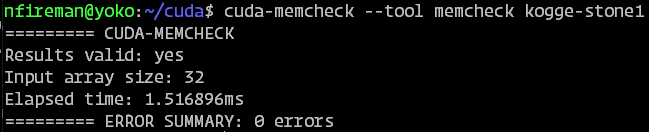
\includegraphics[width=\textwidth]{images/kogge-stone-memcheck.png}
\end{exercise}

\begin{exercise}
Recompile \texttt{kogge-stone1.cu} using the \texttt{-lineinfo} command-line argument (this will cause \texttt{cuda-memcheck} to attach source code line numbers to the errors it finds). Then
use \texttt{cuda-memcheck} to check for race conditions with the \texttt{racecheck} tool. 

You should be prompted with several race condition warnings. Record the program line(s) referenced by each warning message.

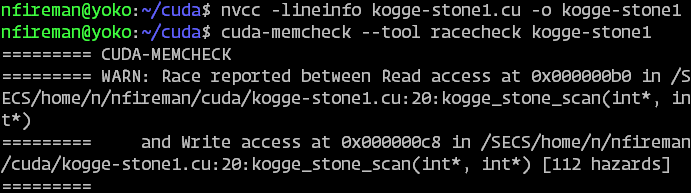
\includegraphics[width=\textwidth]{images/kogge-stone-racecheck.png}
\end{exercise}

The \texttt{racecheck} tool should point to the following line of \texttt{kogge-stone1.cu} as the source of the race condition:

\begin{verbatim}
partials[tid] += partials[tid - stride];
\end{verbatim}

Since the value of \texttt{partials[tid - stride]} may also be updated by a different thread, whether that update occurs before or after the update to \texttt{partials[tid]} will change the effect of the above line of code. This is the source of the race condition detected by \texttt{racecheck}.

To resolve the race condition, we \emph{buffer} the updates to the \texttt{partials} array until the end of each loop iteration. That is, we maintain two arrays, \texttt{partials} and \texttt{partials\_next}, and instead of applying changes directly to \texttt{partials}, we store the new desired value of \texttt{partials[tid]} in \texttt{partials\_next[tid]}. Thus, the above line of code is transformed to the following:

\begin{verbatim}
partials_next[tid] = partials[tid] + partials[tid - stride];
\end{verbatim}

At the end of each loop iteration, we copy \texttt{partials\_next} into \texttt{partials} all at once. This guarantees that the value \texttt{partials[tid - stride]} has a consistent value when it is read by thread \texttt{tid}, regardless of the order in which the threads execute.

\begin{exercise}
Run the \texttt{racecheck} tool on \texttt{kogge-stone2.cu} to verify that a race condition is not detected in this version of the program.
\end{exercise}

\subsubsection*{Additional resources}
\begin{itemize}
    \item "Parallel Prefix Sum (Scan) with CUDA" by Mark Harris.
    
    \url{http://developer.download.nvidia.com/compute/cuda/1.1-Beta/x86_website/projects/scan/doc/scan.pdf}
    
    \resource{resources/scan.pdf}
    
    \item Chapter 8 of "Programming Massively Parallel Processors: A Hands-on Approach", 3rd Edition by David B. Kirk, Wen-mei W. Hwu.
    
    \item Official documentation for \texttt{cuda-memcheck}:
    
    \url{https://docs.nvidia.com/cuda/cuda-memcheck/index.html}
    
    \resource{resources/CUDA\_Memcheck.pdf}
\end{itemize}

\subsection{Mergesort}

Mergesort is a fundamental general-purpose sorting algorithm that is both widely used and relatively simple to implement. In its simplest form, the algorithm first recursively splits an unsorted input array into two equal-sized groups repeatedly until each group has only one element. The second phase of the algorithm is to \emph{merge} two sorted groups into a single larger sorted group, until only one sorted group containing all of the original input values remains. Note that at the start of the second phase, each "group" only has one element each, meaning it is technically sorted. 

Figure \ref{figure/mergesort} demonstrates this procedure on the input array\\ \texttt{\{56,29,35,42,15,41,75,21\}}. The top half of the figure shows the splitting phase and the bottom half shows the merging phase.

\begin{figure}[h!]
    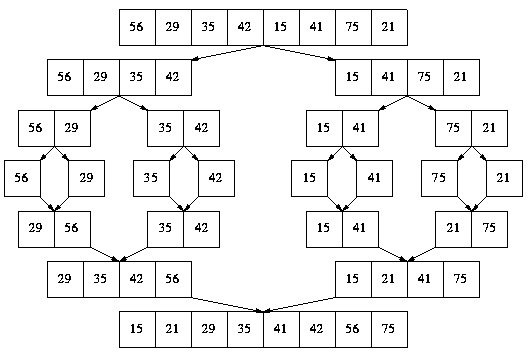
\includegraphics[width=\textwidth]{images/mergesort.png}
    \caption{(source: \url{https://webdocs.cs.ualberta.ca/~holte/T26/merge-sort.html})}
    \label{figure/mergesort}
\end{figure}

\begin{program}

This section presents the program \texttt{merge.cu}, which demonstrates a parallel algorithm for the merging phase of mergesort. The algorithm we will implement was proposed in 2012 for use in the MPI (Message Passing Interface) framework, but we will adapt it accordingly for the CUDA environment. The paper that originally introduced the algorithm is referenced at the end of this section.

First, compile and execute the program. Compare your results to the following screenshot. The remainder of this section will document how this program works.

\textbf{Note:} the justification below is quite complicated and understanding it is not required. It's summarized here as an example of how parallelism can still be applied in practice to nontrivial problems, even when it doesn't seem like it's possible to do so.

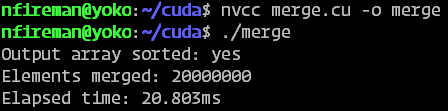
\includegraphics[width=\textwidth]{images/merge-output.png}

\end{program}

\subsubsection{Serial merge}

The first subroutine of our merging kernel will be a function that performs a \emph{serial merge} of two sorted input arrays \texttt{a} (of length \texttt{m}) and \texttt{b} (of length \texttt{n}) into a third output array \texttt{out}:

\begin{verbatim}
__device__ void serial_merge(int *a, int m, int *b, int n, int *out)
\end{verbatim}

The serial merge maintains values \texttt{i} and \texttt{j}, which are the smallest unmerged indices of \texttt{a} and \texttt{b}, respectively. The index \texttt{k} of \texttt{out} that will be merged into next is also maintained. It first merges the smallest of \texttt{a[i]} and \texttt{b[j]} into \texttt{out[k]} (incrementing indices where appropriate) until all values of one input array have been merged. Then, the remaining unmerged values in the other input array are merged to complete the algorithm.

Note the \texttt{\_\_device\_\_} keyword in the declaration to signify that this function will be called from device threads. Our aim in the remainder of the algorithm will be to correctly divide the work of merging two input arrays between many threads, each of which will serially merge distinct subarrays of the inputs into a subarray of the output array.

In particular, we will divide the work of computing the \texttt{m + n} output elements evenly among the allocated threads (recall that the number of threads allocated to a kernel can be computed from the device as \texttt{blockDim.x*gridDim.x}). Each thread can thus determine which output indices it is responsible for. Knowing this, it remains to compute which subarrays of the two input arrays should be merged into each thread's slice of the output array. In other words, we need to be able to work backwards to find the input subarrays that will be merged into a given output subarray.

\subsubsection{Co-rank}

The \texttt{co\_rank} function is the second subroutine in our merging kernel, and is responsible for determining which subarrays of the input will be merged into a given subarray of the output. 

We first observe that for any subarray \texttt{\{out[0], out[1], ..., out[k-1]\}} of the output array, its elements will be obtained from merging subarrays \texttt{\{a[0], a[1], ..., a[i-1]\}} and \texttt{\{b[0], b[1], ..., b[j-1]\}} of the input arrays for some \texttt{i} and \texttt{j}, since input elements are merged from left to right into the output array. In this situation, we say that the input indices \texttt{i} and \texttt{j} are the \emph{co-ranks} of the output index \texttt{k}. Note that \texttt{i + j} must equal \texttt{k}, since subarrays of lengths \texttt{i} and \texttt{j} are merged into a subarray of length \texttt{k}.

Next, suppose we have two output indices \texttt{k0} and \texttt{k1} such that \texttt{k0 < k1}, \texttt{k0} has co-ranks \texttt{i0} and \texttt{j0}, and \texttt{k1} has co-ranks \texttt{i1} and \texttt{j1}. Then since \texttt{\{a[0], ..., a[i0-1]\}} and \texttt{\{b[0], ..., b[j0-1]\}} are merged into \texttt{\{out[0], ..., out[k0-1]\}}, the remaining subarrays \texttt{\{a[i0], ..., a[i1-1]\}} and \texttt{\{b[j0], ..., b[j1-1]\}} must be merged into \texttt{\{out[k0], ..., out[k1-1]\}}.

To see why this fact is useful, we need to apply it to the case where a CUDA thread is assigned to merge into the output indices \texttt{k0} to \texttt{k1 - 1}. In this case, the co-ranks of \texttt{k0} and \texttt{k1} tell us exactly which subarrays of \texttt{a} and \texttt{b} our thread needs to merge into \texttt{\{out[k0], ..., out[k1-1]\}}.

We can now define the behavior of the \texttt{co\_rank} function:

\begin{verbatim}
__device__ int co_rank(int k, int *a, int m, int *b, int n)
\end{verbatim}

If \texttt{k} has co-ranks \texttt{i} and \texttt{j}, then the above call to \texttt{co\_rank} will return \texttt{i}. Note that since \texttt{k=i+j} (as we noted above), \texttt{j} can be computed as \texttt{k-i}, so we only need to explicitly return \texttt{i}.

It remains to develop an algorithm to find the co-ranks of a given index \texttt{k}. In our implementation of \texttt{serial\_merge}, the co-ranks of \texttt{k} will be the values of \texttt{i} and \texttt{j} when \texttt{out[k]} is written to (since at that point, we have merged 
\texttt{\{a[0], a[1], ..., a[i-1]\}} and \texttt{\{b[0], b[1], ..., b[j-1]\}} into \texttt{\{out[0], out[1], ..., out[k-1]\}}). Hence, one way of computing the co-ranks of \texttt{k} would be to "simulate" our serial merge procedure on the entire array.

However, this would be very inefficient for the threads responsible for merging into the end of \texttt{out}. To compute the co-ranks of large output indices in this way, the serial merge would have to process almost all of the elements in both input arrays, one at a time. This work would need to be repeated by every thread assigned to merge into high indices of the output array.

Instead, we will use the fact that both input arrays are sorted to more quickly compute co-ranks without needing to process every input element. We will also use the following characterization of the co-ranks \texttt{i} and \texttt{j} of \texttt{k}: they are indices so that \texttt{i+j == k}, \texttt{a[i-1] <= b[j]}, and \texttt{b[j-1] < a[i]}. 

Using an approach inspired by binary search, the main loop of the \texttt{co\_rank} function finds the co-ranks of \texttt{k} by maintaining candidate indices \texttt{i} and \texttt{j} such that \texttt{i+j} always equals \texttt{k}. At each loop iteration, if \texttt{a[i-1] > b[j]}, then \texttt{j} is increased and \texttt{i} is decreased by the same amount. Otherwise, if \texttt{b[j-1] >= a[i]}, then \texttt{i} is increased and \texttt{j} is decreased by the same amount. Once neither of these inequalities holds, \texttt{i} and \texttt{j} must be the co-ranks of \texttt{k}, and \texttt{i} is returned.

\subsubsection{Parallel merge kernel}

The \texttt{parallel\_merge\_kernel} function ties together the \texttt{serial\_merge} and \texttt{co\_rank} subroutines we have just developed. Each thread computes a unique subarray of the output based on its \texttt{tid} value. The thread then computes the co-ranks \texttt{i} and \texttt{j} of its lowest output index \texttt{k}, as well as the co-ranks \texttt{i\_next} and \texttt{j\_next} of the next thread's lowest output index \texttt{k\_next}. Finally, the thread performs a serial merge of \texttt{\{a[i], ..., a[i\_next-1]\}} and \texttt{\{b[j], ..., b[j\_next-1]\}} into \texttt{\{out[k], ..., out[k\_next-1]\}}.

\begin{exercise}
Try different values of \texttt{THREADS\_PER\_BLOCK} and \texttt{NUM\_BLOCKS} while keeping the original value of \texttt{N=10000000} fixed, and record the runtimes along with the values used. Aim to improve the performance of the unmodified program.
\end{exercise}

\subsubsection*{Additional resources}
\begin{itemize}
    \item "Efficient MPI Implementation of a Parallel, Stable Merge Algorithm" by Christian Siebert, Jesper Larsson Träff (EuroMPI 2012).
    
    \url{https://link.springer.com/chapter/10.1007%2F978-3-642-33518-1_25}
    
    \resource{resources/MPI\_Mergesort.pdf}

    \item Documentation for the \texttt{merge} operation in the \texttt{moderngpu} CUDA library:
    
    \url{https://moderngpu.github.io/merge.html}
    
    \resource{resources/moderngpu\_merge.pdf}
    
    \item Chapter 11 of "Programming Massively Parallel Processors: A Hands-on Approach", 3rd Edition by David B. Kirk, Wen-mei W. Hwu.
    
    \item  "Designing efficient sorting algorithms for manycore GPUs" by N. Satish, M. Harris and M. Garland (2009 IEEE International Symposium on Parallel \& Distributed Processing).
    
    \url{https://mgarland.org/files/papers/gpusort-ipdps09.pdf}
    
    \resource{resources/gpusort-ipdps09.pdf}
\end{itemize}

\subsection{Sparse matrix-vector multiplication}

This section will make extensive use of \emph{matrices}, which is the mathematical name for two-dimensional arrays. The following C code defines a $3$ by $4$ matrix \texttt{A} (meaning that \texttt{A} has $3$ rows and $4$ columns):

\begin{verbatim}
int A[3][4] = { { 1, 2, 3, 4 }, 
                { 3, 4, 5, 6 },
                { 5, 6, 7, 8 } };
\end{verbatim}  

This section will present a solution for the \emph{matrix-vector multiplication} problem, which is defined as follows. Suppose we have an \texttt{m} by \texttt{n} matrix \texttt{A} and a vector \texttt{x} of length \texttt{n}. Then the matrix-vector product \texttt{A * x} is a vector \texttt{y} of length \texttt{m}, where \texttt{y[i]} is the dot product of the \texttt{i}-th row of \texttt{A} with \texttt{x}. In other words, for \texttt{0 <= i < m}:

\begin{verbatim}
y[i] = A[i][0]*x[0] + A[i][1]*x[1] + ... + A[i][n-1]*x[n-1];
\end{verbatim}

In this section, we will also additionally assume that the input matrix \texttt{A} is \emph{sparse}; a matrix is said to be sparse if most of its values are zero. There's no precise cutoff for when a matrix is sparse or not, but in practice it generally means that only a small (constant) number of elements are nonzero per row or column.\footnote{If you're familiar with asymptotic notation, then assuming an $m$ by $n$ matrix is sparse usually means that at most $O(m + n)$ of its $mn$ elements are nonzero.} 

Storing a sparse matrix as a two-dimensional array (like in the above code) is often inefficient, since the vast majority of the memory is going to be used to store zero-valued elements. To take better advantage of sparsity, \emph{sparse matrix encodings} have been developed to store sparse matrices in memory more efficiently than with a two-dimensional array.

This section will define the \emph{Compressed Sparse Row} (CSR) encoding for sparse matrices. For a given sparse matrix \texttt{A}, the aim of the CSR scheme is to encode the positions and values of just the nonzero elements of \texttt{A}; any element left unencoded is guaranteed to be \texttt{0}. Assuming that \texttt{A} is sufficiently sparse, this will save significant memory over the traditional array encoding of \texttt{A}.

Suppose we have the following matrix:
\begin{center}
$A = 
\begin{bmatrix}
2 & 0 & 0 & 1 \\
0 & 4 & 7 & 5 \\
0 & 0 & 0 & 0 \\
3 & 0 & 2 & 0 \\
\end{bmatrix}$
\end{center}

The CSR compression scheme uses three arrays to encode the matrix $A$.
The first array \texttt{data} will simply be the nonzero elements of $A$ listed in order, where we read the top row left-to-right, and continue through the rows top-to-bottom:

\begin{verbatim}
float data[7] = {2, 1, 4, 7, 5, 3, 2};
\end{verbatim}

The second array \texttt{col\_index} will be the same size as \texttt{data}, and \texttt{col\_index[i]} will be the column index of the corresponding nonzero value \texttt{data[i]}. For example, \texttt{data[2]} references the \texttt{4} belonging to column index 1 of $A$, so \texttt{col\_index[2]} should be $1$.

\begin{verbatim}
int col_index[7] = {0, 3, 1, 2, 3, 0, 2};
\end{verbatim}

Since \texttt{col\_index} encodes the column index of each nonzero value of $A$, we could complete the encoding by defining a similar array \texttt{row\_index} which encodes the row index of each nonzero value:

\begin{verbatim}
int row_index[7] = {0, 0, 1, 1, 1, 3, 3};
\end{verbatim}

Note that the entries in \texttt{row\_index} will correspond to the two values in row 0, then the three values in row 1, then the two values in row 3. This is due to the order in which the nonzero values of $A$ were read into \texttt{data}. To take advantage of this, we can instead define the array \texttt{row\_ptr}, which only records the first index of \texttt{data} corresponding to each row:

\begin{verbatim}
int row_ptr[4] = {0, 2, 5, 5};
\end{verbatim}

Here we have that \texttt{row\_ptr[1]} is 2 since \texttt{data[2]} is the first nonzero value on row 1. Likewise, \texttt{row\_ptr[0]} is 0 and \texttt{row\_ptr[3]} is 5. In the case where a row is all zeros (e.g. row 2), its value will be equal to the next value in \texttt{row\_ptr}. Thus, \texttt{row\_ptr[2] == row\_ptr[3] == 5}.

This definition yields the following invariant: the nonzero values of $A$ in row $i$ lie between the indices \texttt{row\_ptr[i]} and \texttt{row\_ptr[i+1]-1} of \texttt{data}. If row $i$ is all zeros, then we can deduce this from the fact that \texttt{row\_ptr[i]} will equal \texttt{row\_ptr[i+1]}.

For convenience, an extra element is often added to the end of \texttt{row\_ptr} so that the above invariant still holds for the last row of $A$. The extra element will always be equal to the length of \texttt{data}:

\begin{verbatim}
int row_ptr[5] = {0, 2, 5, 5, 7};
\end{verbatim}

Applying the invariant to row 3 tells us that the nonzero elements of row 3 lie between indices \texttt{row\_ptr[3] == 5} and \texttt{row\_ptr[4]-1 == 6} of \texttt{data}. This correctly points to the elements \texttt{3} and \texttt{2} on the last row of $A$.

\begin{exercise}
Suppose a sparse matrix of \texttt{float} values \texttt{A} has 1000 rows, 1000 columns, and that \texttt{A} has exactly $2$ nonzero entries per row. Compare the amount of memory needed to store \texttt{A} as a traditional two-dimensional array to the memory needed to store it as a CSR-encoded matrix. Assume that \texttt{float} and \texttt{int} values each use $4$ bytes of memory.
\end{exercise}

\begin{program}
The program \texttt{spmv-csr.cu} implements matrix-vector multiplication for CSR-encoded matrices. The kernel function \texttt{spmv\_csr} is similar to the kernel function found in \texttt{dot-product-parallel.cu} (which computed the dot product of two vectors), since matrix-vector multiplication is defined as a series of dot products.

The following code block uses what has been previously established about the CSR encoding to compute the dot product of the row of index \texttt{row} of \texttt{A} with the input vector \texttt{x}:

\begin{verbatim}
float partial = 0;
int min_idx = row_ptr[row];
int max_idx = row_ptr[row + 1];
for (int i = min_idx; i < max_idx; i++) {
  partial += data[i] * x[col_index[i]];
}    
y[row] = partial;
\end{verbatim}

First, subarrays of \texttt{data} and \texttt{col\_index} corresponding to row index \texttt{row} are computed using \texttt{row\_ptr}. Each element in this subarray of \texttt{data} is then multiplied with the corresponding value of \texttt{x} and added to the intermediate result \texttt{partial}. At the end of the loop, \texttt{partial} contains the dot product, and it is stored in the output vector \texttt{y}.
\end{program}

\begin{exercise}
Compile and execute \texttt{spmv-csr.cu}. Improve the performance of the program by trying several different values for \texttt{THREADS\_PER\_BLOCK} and \texttt{NUM\_BLOCKS}. Note the runtime for each pair of values tried.
\end{exercise}

\begin{exercise}
The value \texttt{NONZERO\_ELTS\_PER\_ROW} controls the number of nonzero elements in each row of the generated input matrix. To see how the CSR encoding performs when the input matrix is less sparse, record the program runtime when the elements per row is increased to 100, 250, and 500.
\end{exercise}

\subsubsection*{Additional resources}
\begin{itemize}
    \item "Efficient Sparse Matrix-Vector Multiplication on CUDA" by Nathan Bell, Michael Garland.
    
    \url{https://www.nvidia.com/docs/IO/66889/nvr-2008-004.pdf}
    
    \resource{resources/nvr-2008-004.pdf}
    
    \item Chapter 10 of "Programming Massively Parallel Processors: A Hands-on Approach", 3rd Edition by David B. Kirk, Wen-mei W. Hwu.

\end{itemize}

\end{document}
